\chapter{Methoden}   \label{ch_3}
In diesem Kapitel wird die empirische Bearbeitung der Hypothesen dargestellt. Zunächst wird die erhobene Stichprobe beschrieben, gefolgt von der Erläuterung der Erhebungsmethode, Stichprobenauswahl und das Erhebungsdesign. Darauf folgend wird auf die Operationalisierung der Konstrukte eingegangen. In folgendem Zuge wird die Untersuchungsdurchführung konkretisiert und abschließend wird auf die Auswertungsmethode eingegangen.

\section{Stichprobenbeschreibung} \label{sec_3.1}
% schreiben wie viele insgesamt und wie bereinigt
Mittels eines Onlinefragbogens wurde die Stichprobe mit $N = 432$ erfasst. Mit $n = 305$ (70.60\%) bilden weibliche Teilnehmer den größten Teil der Gesamtstichprobe ab. Männliche Teilnehmer betrugen 28.9\% ($n = 125$) der Befragten. Des Weiteren gaben 0.5\% ($n = 2$) der Probanden an ein diverses Geschlecht zu haben. Das Durchschnittsalter der Befragten lag bei $M = 33.52$ Jahren ($SD = 13.67$). Eine grafische Darstellung der Altersverteilung ist in Abbildung~\ref{Histogramm Altersverteilung} zu sehen. An ihr lässt sich ablesen, dass der jüngste Teilnehmer 18 Jahre alt war, der älteste betrug ein Alter von 77 Jahren. Es handelt sich dabei um eine unimodale und rechtsschiefe verteilung. \begin{figure}[htb]
    \centering
        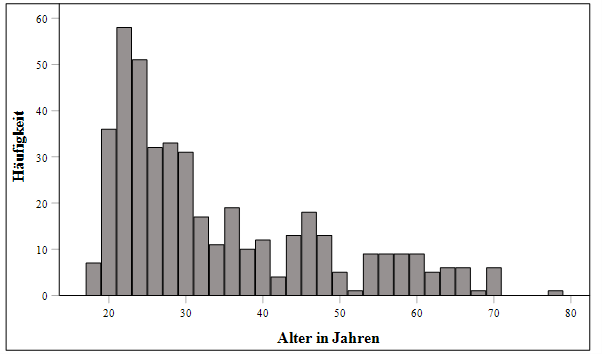
\includegraphics[width=0.8\linewidth]{Histogramm - Altersverteilung.png}
        \caption[Histogramm Altersverteilung]{Histogramm für die Altersverteilung.}
        \label{Histogramm Altersverteilung}
\end{figure}





\section{Untersuchungsdesign}  \label{sec_3.2}
Präregistrierung \\ %im Rahmen dessen gibt es weitere 4 Studien und NUR nennen was die erhoben
Feld-Laborstudie\\
genutzte Methode \\
Design \\
warum Online gemacht \\
effekte\\
randomiesiert und warum \\
Anfallende Stichprobe (Ad-hoc-Stichprobe)
quantitativer Forschungsansatz mittels Onlinefragbogen


\section{Operationalisierung der Konstrukte}    \label{sec_3.3}
Damit die Teilnehmer unvoreingenommen die, der Wahrheit ähnelten, fiktiven Fallvignetten bewerten konnten, begann der Fragebogen mit zwei zufällig zugeodneten Vignetten, die psychische oder sexualisierte Gewalt behandelten. Darauf folgte die deutsche Version der Skala zur Erfassung der Akzeptanz von Gewaltmythen. Im Anschluss befand sich eine umfangreiche Testbatterie mit vier Skalen um physische wie verbale Aggression, den Ärger und das Misstrauen zu messen. Abschließend wurden die soziodemografischen Daten wie Alter, Geschlecht, kultureller Hintergrund, Bildungsstand, berufliche Situation und das Einkommen erfragt.

Mithilfe der Fallvignetten zur häuslichen Gewalt wurde die Verantwortungszuschreibung erhoben. Insgesamt wurden 16 unterschiedliche Vignetten generiert, um vier verschiedene Variablen messen zu können. Bei diesen Variablen handelte es sich umd die Gewaltart (psychisch oder sexualisiert), das Geschlecht (männlich oder weiblich), den sozioökonomischen Status (hoch oder niedrig) und um den kulturellen Hintergrund (deutsch oder arabisch). Über einen Schiberegler konnten die Probanden die relative Verantwortung von Opfer und Täter bewerten. Die Codierung verlief vom kleinstmöglichen Punktewert auf der linken Seit bis zum größtmöglichen Punktewert auf der rechten Seite (Codierung 1-101). 

Die Akzeptanz von häuslichen Gewaltmythen wurden mithilfe der deutschen Übersetzung des englischen Domestic Violence Myth Acceptance Scale (DVMAS) \parencite{Peters2003} unternommen. Bis auf das letzte Item sind alle übrigen 17 Items als Aussagen vormuliert und wurden mithilfe einer siebenstufigen Skala, von 1 = \enquote{Stimme überhaupt nicht zu} bis 7 = \enquote{Stimme völlig zu}, beantwortet. Für die deutsche Übersetzung des DVMAS liegt bislang noch keine Validierung vor. Da es hierbei um eine Sinngemäße Übersetzung handelt wird die Reliabilität und Validität des originalen DVMAS herangezogen. Die Reliabilität von Cronbachs-\textalpha~=~.88 liegt in einem sehr gute Bereich. Des Weiteren liegt auch eine gute Validität vor, zumal der DVMAS signifikante Korrelationen mit den folgenden vier theoretisch ähnelnden Skalen aufweist: Attitude Towards Women, Rape Myth acceptance scale, Sex Role Stereotypes und Attitude Towards Wife Abuse \parencite{DVMAS_Peters}.

Das letzte erhobene Konstrukt Aggression wurde mithilfe des Deutschen Aggressionsfragebogens erfasst. Dieser umfasst 29 Items verteilt auf den folgenden vier Subskalen: physische Aggression, verbale Aggression, Ärger und Misstrauen. Die als Aussage formulierten Items wurden anhand einer vier-stufigen Likertskala von 1 = \enquote{trifft nich zu} bis 4 = \enquote{trifft voll zu} beantwortet. Die Validität des Fragebogens wurde durch die signifikante Korrelationen mit Aggressivität, generalisierter Selbstwert, Ärger, Ärgerkontrolle und Neurotizismus festgestellt. Die Reliabilität variiert zwischen \textalpha~=~.62 und \textalpha~=~.82 (Cronbachs-\textalpha der Subskalen) und weißt eine Retestreliabilität von Cronbachs-\textalpha~=~.73\parencite{Aggressionsfragebogen}.

\textbf{Manipulationscheck}
Fragestellung und Hypothesen


\section{Untersuchungsdurchführung}   \label{sec_3.4}
Über den Zeitraum vom 04.06.2022 bis 27.06.2022 erstreckte sich die Datenerhebung. Der über SoSci-Survey erstellte Fragebogen wurde primär über den Messenger-Dienst WhatsApp, aber auch über Instagram, Facebook, Signal und Telegram verbreitet, mit der Bitte der Verbreitung, um eine möglichst große Stichprobe zu erreichen. Die Mindeststichprobengröße von 395 wurde mithilfe des kostenlosen Tools G*Power ermittelt. %G*Power (https://bjoernwalther.com/eine-kurze-einfuehrung-in-gpower/)

Im Einführungstext, zu Beginn der Befragung, wurden Auskünfte über die 15 minütige Bearbeitungszeit, wie auch die garantierte Anonymität der Probanden aufgeklärt. Die Teilnehmer wurden zudem darauf hingewiesen, dass die Teilnahme der Befragung freiwillige ist. Bevor auf die nächste Seite weitergeklickt werden konnte, wurde mithilfe einer zu beantworteten Frage sichergestellt, dass die Person den Einleitungstext verstanden hat und mit der Befragung einverstanden ist. Auf der anschließenden Seite folgte die Aufgabenerklärung für die Fallvignetten, wie eine kleine Aufklärung diesbezüglich. Jeweils nach jeder dargebotener Vignette folgten vier Fragen, zur überprüfung der Manipulation, die bereits in ~\ref{sec_3.3} aufgefasst wurden. Anschließend folgten die deutsche Übersetzung des DVMAS und der Deutsche Aggressionsfragebogen. Zum Schluss wurden die Probanden gebeten einige kurze Angaben zu ihrer Person zu geben, woraufhin eine letzte Nachfrage der gewissenhaften Durchführung folgte. Damit endete der für die Forschenden wichtige Teil der Befragung. Auf einer daran anschließenden Seite wurden Informationen und Kontaktdaten für Betroffene von häuslicher Gewalt gewährleistet. 

Potenzielle Störvariablen konnten während der Untersuchungsdurchführung nicht kontrolliert werden. Anhand der Onlinebefragung lag die Entscheidung, zu welchem Zeitpunkt, an welchem Ort und unter welchen Bedingungen die Befragung bearbeitet wurde, bei den Teilnehmern selbst.


\section{Auswertungsmethode}    \label{sec_3.5}
SPSS ausgewertet \\ %was umgepolt wurde: Variablen wurden so umkodiert, dass der betroffenen Person stets der Zahlenwert 101 sprich der vollen Verantwortung zugeschrieben wurde (GP2,3,6    GS1,4,7) + Aggro 14,22
% Vorbereitung der Daten: wieviele wurden rausgeschmissen
deskriptive \\ % Lage, Streuung, Median, Modus, Mittelwert, SD
hypothesen \\ % das aus präregistrierung: gerichtet, unterschied, tests
% H3, weil Moderatorviariable hat wurde auf SPSS mit dem plug-in PROCESS berechnet
erwähnen, dass Vorraussetzung gibt und werden später geprüft

auf 1-2 items eingehen wenn über FB geschrieben wird